
 \documentclass[12pt]{article}
\usepackage{graphicx}
\usepackage{booktabs}
 \usepackage{makecell}
 \usepackage{float}
 \newcommand{\diff}{\,\mathrm{d}}
\usepackage[margin=1in]{geometry}
\usepackage{fancyhdr}
\pagestyle{fancy}
\usepackage{extarrows}
\usepackage{breqn}

\newcommand{\N}{\mathbb{N}}
\newcommand{\Z}{\mathbb{Z}}
\newcommand{\trans}{^{\mathrm T}}
\usepackage{amssymb}
\usepackage[table]{xcolor}
\usepackage{bm}
\usepackage{array}
\usepackage{mathtools}
\usepackage[english]{babel}
\usepackage{natbib}
\usepackage{url}
\usepackage[utf8x]{inputenc}
\usepackage{amsmath}
\usepackage{graphicx}
\graphicspath{{images/}}
\usepackage{parskip}
\usepackage{fancyhdr}
\usepackage{vmargin}
\usepackage[font={bf, footnotesize}, textfont=md]{caption}
\usepackage{amsmath,amsthm,amssymb}


\newenvironment{theorem}[2][Theorem]{\begin{trivlist}
\item[\hskip \labelsep {\bfseries #1}\hskip \labelsep {\bfseries #2.}]}{\end{trivlist}}
\newenvironment{lemma}[2][Lemma]{\begin{trivlist}
\item[\hskip \labelsep {\bfseries #1}\hskip \labelsep {\bfseries #2.}]}{\end{trivlist}}
\newenvironment{exercise}[2][Exercise]{\begin{trivlist}
\item[\hskip \labelsep {\bfseries #1}\hskip \labelsep {\bfseries #2.}]}{\end{trivlist}}
\newenvironment{reflection}[2][Reflection]{\begin{trivlist}
\item[\hskip \labelsep {\bfseries #1}\hskip \labelsep {\bfseries #2.}]}{\end{trivlist}}
\newenvironment{proposition}[2][Proposition]{\begin{trivlist}
\item[\hskip \labelsep {\bfseries #1}\hskip \labelsep {\bfseries #2.}]}{\end{trivlist}}
\newenvironment{corollary}[2][Corollary]{\begin{trivlist}
\item[\hskip \labelsep {\bfseries #1}\hskip \labelsep {\bfseries #2.}]}{\end{trivlist}}
\DeclareMathOperator{\tr}{tr}
\DeclareMathOperator{\rank}{rank}
\DeclareMathOperator{\Span}{span}
\DeclareMathOperator{\row}{row}
\DeclareMathOperator{\col}{col}
\DeclareMathOperator{\range}{range}
\DeclarePairedDelimiterX{\inp}[2]{\langle}{\rangle}{#1, #2}
\DeclareMathOperator{\Proj}{Proj}
\DeclareMathOperator{\trace}{trace}
\newcommand{\Her}{^{\mathrm H}}
\DeclareMathOperator{\diag}{diag}
\makeatletter 
    \newcommand\fcaption{\def\@captype{table}\caption}
\makeatother
\setmarginsrb{3 cm}{2.5 cm}{3 cm}{2.5 cm}{1 cm}{1.5 cm}{1 cm}{1.5 cm}
\setlength\parindent{1em}

\title{Short Report: Large Amplitude Pendulum}                             % Title
\author{Chen Ang}                               % Author
\date{\today}                                           % Date

\makeatletter
\let\thetitle\@title
\let\theauthor\@author
\let\thedate\@date
\makeatother

\pagestyle{fancy}
\fancyhf{}
\rhead{\theauthor}
\lhead{\thetitle}
\cfoot{\thepage}

\begin{document}

%%%%%%%%%%%%%%%%%%%%%%%%%%%%%%%%%%%%%%%%%%%%%%%%%%%%%%%%%%%%%%%%%%%%%%%%%%%%%%%%%%%%%%%%%

\begin{titlepage}
    \centering
    \vspace*{0.5 cm}
    
\includegraphics[scale = 0.75,width=6cm]{CUHK}\\[1.0 cm]   % University Logo
    \textsc{\large The Chinese University of Hong Kong, Shenzhen}\\[2.0 cm]   % University Name
    \textsc{\Large PHY 1002}\\[0.5 cm]               % Course Code
    \textsc{\large Physics Laboratory}\\[0.5 cm]               % Course Name
    \rule{\linewidth}{0.2 mm} \\[0.4 cm]
    { \huge \bfseries \thetitle}\\
    \rule{\linewidth}{0.2 mm} \\[1.5 cm]
    
    \begin{minipage}{0.4\textwidth}
        \begin{flushleft} \large
            \emph{Author:}\\
            \theauthor
            \\
            \emph{Group Number:} \\
            Group 1
            \end{flushleft}
            \end{minipage}~
            \begin{minipage}{0.4\textwidth}
            \begin{flushright} \large
            \emph{Student Number:} \\
            118010009                                   % Your Student Number
            \\
            \emph{Experiment Date:}\\
            September 27, 2019
        \end{flushright}
    \end{minipage}\\[2 cm]
    
    {\large \thedate}\\[2 cm]
 
    \vfill
    
\end{titlepage}

%%%%%%%%%%%%%%%%%%%%%%%%%%%%%%%%%%%%%%%%%%%%%%%%%%%%%%%%%%%%%%%%%%%%%%%%%%%%%%%%%%%%%%%%%
%%%%%%%%%%%%%%%%%%%%%%%%%%%%%%%%%%%%%%%%%%%%%%%%%%%%%%%%%%%%%%%%%%%%%%%%%%%%%%%%%%%%%%%%%

\tableofcontents
\pagebreak


%%%%%%%%%%%%%%%%%%%%%%%%%%%%%%%%%%%%%%%%%%%%%%%%%%%%%%%%%%%%%%%%%%%%%%%%%%%%%%%%%%%%%%%%%

\rmfamily

\section{Introduction}

This experiment is to validate the following important special case of the \textit{conservation of angular momentum}:
\\
\begin{thm}[]
	If a rigid body is rotating around a fixed axis O, and experiences no external net torque, then its angular momentum is given by
	$$
	L = I\omega
	$$
	and conserved, where I is the moment of inertia of the body, $\omega$ the angular velocity, both about axis O.
\end{thm}
In this experiment, we calculated the angular momentum as well as the angular kinetic energy of a torque-free system, by measuring the moment of inertia and angular velocity of the system before and after a collision process. The initial and final values were finally compared to verify the conservation of angular momentum, as well as the conservation of rotational kinetic energy.

\section{Theory}

\subsection{Conservation of Angular Momentum}
In the experiment, a ring and a disk are dropped on top of a rotating disk. Assuming the external torque being negligible, \textbf{Theorem 1} asserts that the angular momentum of the system before and after the collison should be constant. That is,
$$
L_i=I_i\omega_i=I_f\omega_f=L_f
$$
where
$$
\begin{aligned}
I_i,I_f&\ \ \text{ are the initial and final moment of inertia of the system},\\
\omega_i,\omega_f&\ \ \text{ are the initial and final angular velocity of the system}.
\end{aligned}
$$
Also, in both experiment groups, the initial moment of inertia is exactly that of the first disk (mass $M_d$, radius $R_d$):
$$
I_i = I_{d}=\frac{1}{2}R_d^2M_d.
$$
\subsubsection{Dropping Ring}
The moment of inertia of a ring (mass $M_r$, inner radius $R_1$, outer radius $R_2$) about the central axis is obtained by the following formula
$$
I_r = \frac12 M_r(R_1^2+R_2^2+x^2).
$$
Then
$$
I_f = I_i + I_r=\frac12 \left(M_r(R_1^2+R_2^2+x^2)+R_d^2M_d\right)
$$
where $x$ is the distance of the center of the ring from the rotational axis.
\subsubsection{Dropping Disk}
In the case of a dropping disk, the final moment of inertia is the sum of that of two disks:
$$
I_f = I_i + I_d'= \frac12(R_d^2M_d+(R'_d)^2M_d').
$$
where $R'_d$ is the radius of the Dropped Disk, $M_d'$ the mass.
\subsection{Conservation of Rational Kinetic Energy}
The conservation of the rotational kinetic energy was also investigated. The ratational kinetic enery of each system, $\text{KE}$, is given by
$$
\text{KE} = \frac{1}{2}I\omega^2.
$$
\section{Procedures}
\subsection{Parameters Collection}
Several important physical parameters mentioned in Section \textbf{2.3} should be collected ahead of the experiment (See \textbf{Table 1}). It should be noted that if the moment of inertia of the pulley is not neglibliy small compared to the Rotating Disk, it should be added to the moment of inertia of the Rotating Disk. In this experiment, the moment of inertia of the pulley was taken into acount for a positive result.

\begin{table}[!htb]
	\centering
	\begin{tabular}{@{}lllll@{}}
		\cmidrule(r){1-4}
		Ring & Dropped Disk & Rotating Disk & Pulley &  \\ \cmidrule(r){1-4}
		\multicolumn{1}{l|}{mass $M_r$} & \multicolumn{1}{l|}{mass $M_d$} & \multicolumn{1}{l|}{mass $M_d'$} & mass $M_p$ &  \\
		\multicolumn{1}{l|}{inner radius $R_1$} & \multicolumn{1}{l|}{radius $R_d$} & \multicolumn{1}{l|}{radius $R_d'$} & radius $R_p$ &  \\
		\multicolumn{1}{l|}{outer radius $R_2$} & \multicolumn{1}{l|}{} & \multicolumn{1}{l|}{} &  &  \\ \cmidrule(r){1-4}
	\end{tabular}
\caption{Parameters Collected before the Experiment}
\end{table}

\subsection{Setup}
A Rotary Motion Sensor was mounted to the support rod and connected to the 550 Universal Interface. Next, a pulley was attached to the Rotary Motion Sensor. Disk 1 (Rotating Disk) was then attached to the pulley. After this had been done, a level check of the disk was performed to avoid periodic wobbling due to gravity. Pre-run (spin at around $3$ rad/s) the disk and adjust the stand until the angular velocity of the disk no longer fluctuates periodically.

\subsection{Ring-on-Disk Collision}
Having activated the Rotary Motion Sensor, a torque was applied manually to the Rotating Disk so that it rotated at $20$-$30$ rad/s. After the rotation stabilized, the Ring was held $2$-$3$ mm above the center of the Rotating Disk. The Ring was then released and struck the Rotating Disk, resulting in a Ring-on-Disk system spinning together at a lower angular velocity. Wait until the system settles, then record the minimum distance, $D$, between the Ring and the edge of the disk. The off-center distance, $x,$ is then computed by
$$
x = R_d-R_2-D.
$$
The entire procedure was repeated thrice.

Making sure that the released ring lands approximately at the center of the disk is vital for good results afterward, as the error in the measurement of the minimum-from-edge distance $d$ is likely to be significant. To ensure a good landing location,
It is advised that the experimenter observes the relative position of the Ring and the disk from the top down. It is also suggested that the height at which the Ring is released should not be too high. Releasing at a lower height can also help minimize any external torque caused by friction.

\subsection{Disk-on-Disk Collision}
A similar procedure to that in Ring-on-Disk was performed for Disk-on-Disk collision. With the troughs on two disks, it was easier in this case to let the collision happen at the center of the Rotating Disk. However, it is still necessary to release the Dropped Disk as low as possible in order to minimize undesired frictional drag.

\section{Data and Error}
\subsection{Measured Quantities}
The error in measured variables mainly comes from the uncertainty due to the resolution limit of the measuring instruments. Hence, it is reasonable to adopt the highest resolution of the measuring instruments as the error of each measured variable. 

The following table records all measuring instruments utilized in the experiment, along with their errors (resolutions), and measured variables.
\begin{table}[!htb]
	\centering
	\begin{tabular}{@{}lllll@{}}
		\toprule
		Instrument & $\delta$ & Measured Quantities &  &  \\ \midrule
		\multicolumn{1}{l|}{Rotary Motion Sensor} & \multicolumn{1}{l|}{0.002 rad/s} & $\omega$ &  &  \\ \cmidrule(r){1-3}
		\multicolumn{1}{l|}{Electronic Balance} & \multicolumn{1}{l|}{0.01 g} & $R_1,R_2,R_d,R_d',R_p$ &  &  \\ \cmidrule(r){1-3}
		\multicolumn{1}{l|}{Caliper} & \multicolumn{1}{l|}{0.0025 cm} & $M_r,M_d,M_d',M_p, D$ &  &  \\ \bottomrule
	\end{tabular}
\caption{Instrumental Error in Measured Quantities}
\end{table}

Raw data of directly measured variables are given below.
\begin{table}[!htb]
	\centering
	\begin{tabular}{@{}lllll@{}}
		\cmidrule(r){1-4}
		Object & $M$ (g) & $R_{\text{out}}$ (cm) & $R_{\text{in}}$ (cm) &  \\ \cmidrule(r){1-4}
		\multicolumn{1}{l|}{Ring} & \multicolumn{1}{l|}{469.17$\ \pm 0.01$} & \multicolumn{1}{l|}{3.8200$\ \pm 0.0025$} & 2.6350$\ \pm 0.0025$ &  \\
		\multicolumn{1}{l|}{Rotating Disk} & \multicolumn{1}{l|}{122.24$\ \pm 0.01$} & \multicolumn{1}{l|}{4.7625$\ \pm 0.0025$} &  &  \\
		\multicolumn{1}{l|}{Dropped Disk} & \multicolumn{1}{l|}{120.39$\ \pm 0.01$} & \multicolumn{1}{l|}{4.7575$\ \pm 0.0025$} &  &  \\ \cmidrule(r){1-4}
	\end{tabular}
\caption{Physical Quantities}
\end{table}

\begin{table}[!htb]
	\centering
	\begin{tabular}{@{}lllll@{}}
		&  &  &  &  \\ \cmidrule(r){1-4}
		Dropped Object & $\omega_i$ (rad/s) & $\omega_f$ (rad/s) & $x$ (cm) &  \\ \cmidrule(r){1-4}
		\multicolumn{1}{l|}{Ring (run 1)} & \multicolumn{1}{l|}{26.028$\ \pm 0.002$} & \multicolumn{1}{l|}{5.592$\ \pm 0.002$} & 0.0625$\ \pm 0.0025$ &  \\
		\multicolumn{1}{l|}{Ring (run 2)} & \multicolumn{1}{l|}{23.389$\ \pm 0.002$} & \multicolumn{1}{l|}{5.121$\ \pm 0.002$} & 0.0925$\ \pm 0.0025$&  \\
		\multicolumn{1}{l|}{Ring (run 3)} & \multicolumn{1}{l|}{23.892$\ \pm 0.002$} & \multicolumn{1}{l|}{5.199$\ \pm 0.002$} & 0.1075$\ \pm 0.0025$ &  \\
		\multicolumn{1}{l|}{Disk} & \multicolumn{1}{l|}{26.044$\ \pm 0.002$} & \multicolumn{1}{l|}{12.928$\ \pm 0.002$} &  &  \\ \cmidrule(r){1-4}
	\end{tabular}
\caption{Collision Data: Angular Velocity and Distance off Center}
\end{table}

\begin{figure}[!htb]
	\centering
	\begin{minipage}{.5\textwidth}
		\centering
		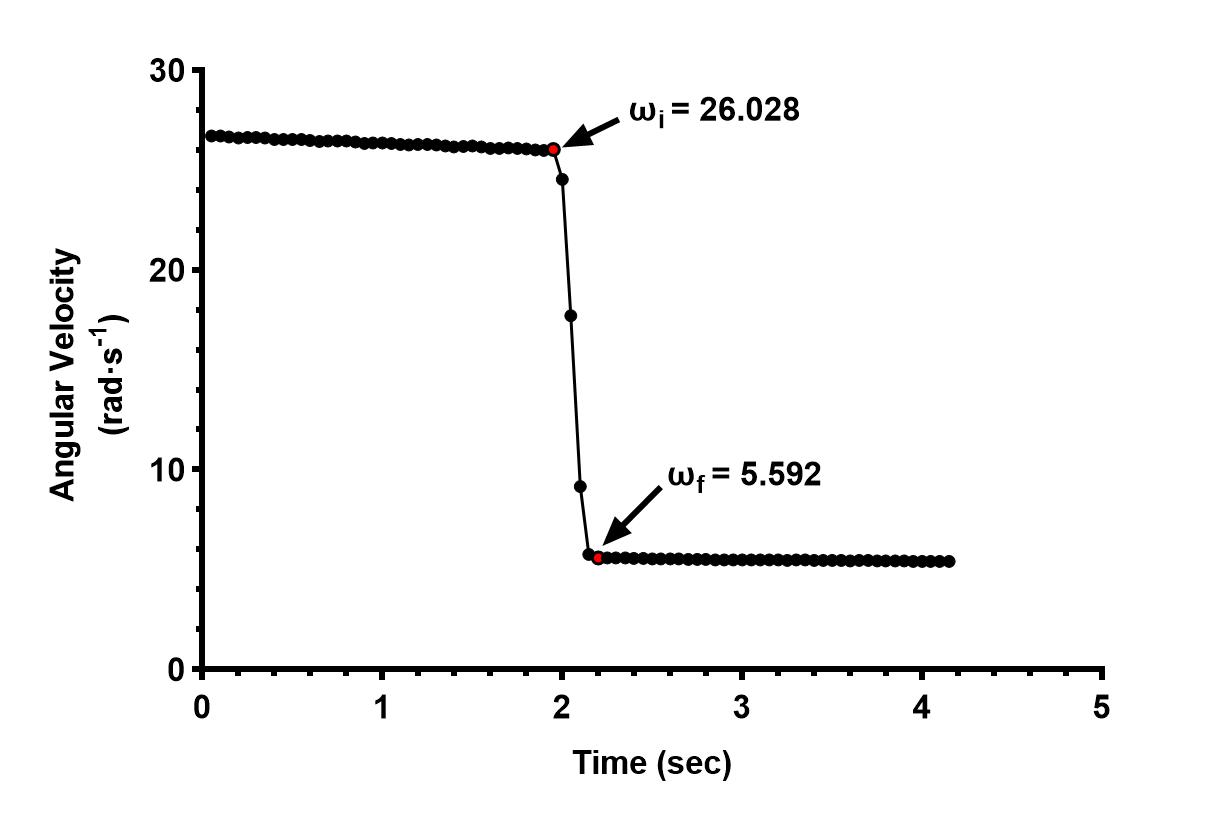
\includegraphics[width=\linewidth]{r1}
		\captionof{figure}{Ring (run 1)}
		\label{fig:test1}
	\end{minipage}%
	\begin{minipage}{.5\textwidth}
		\centering
		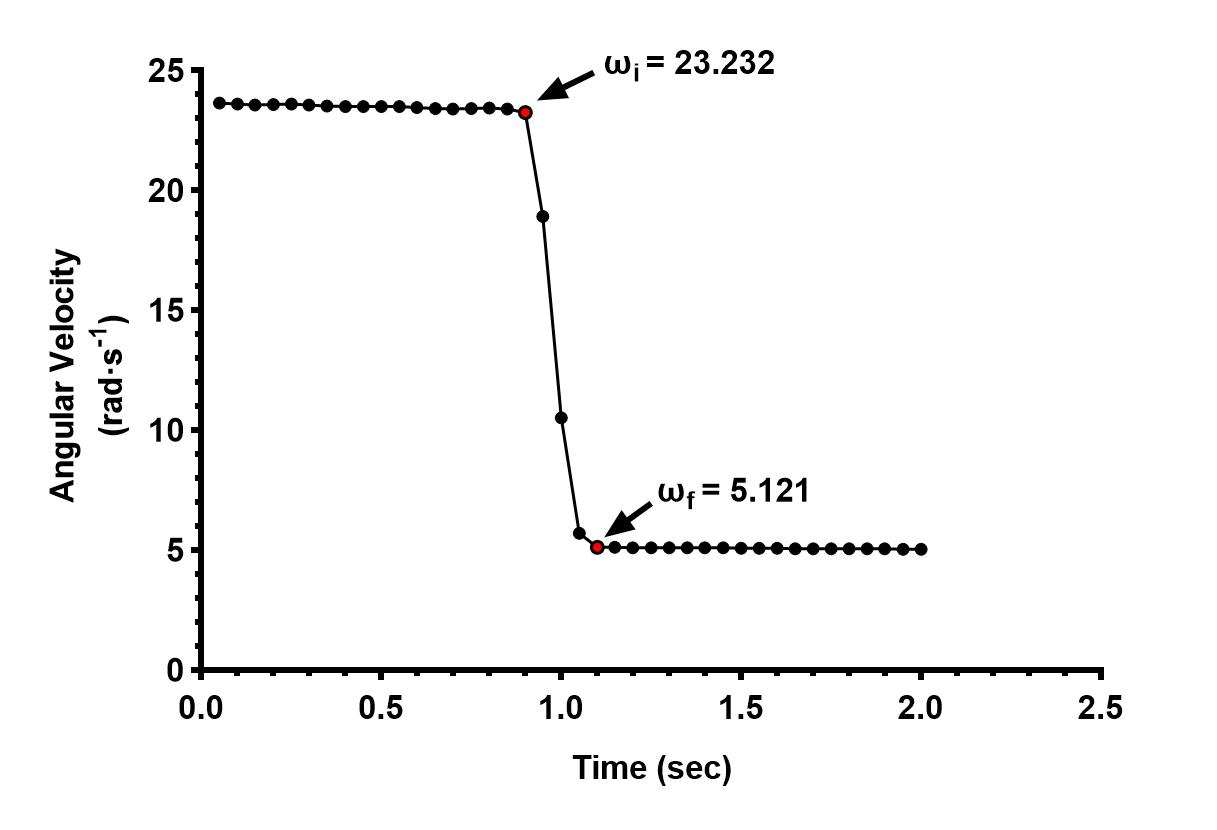
\includegraphics[width=\linewidth]{r2}
		\captionof{figure}{Ring (run 2)}
		\label{fig:test2}
	\end{minipage}\\
	\begin{minipage}{.5\textwidth}
	\centering
	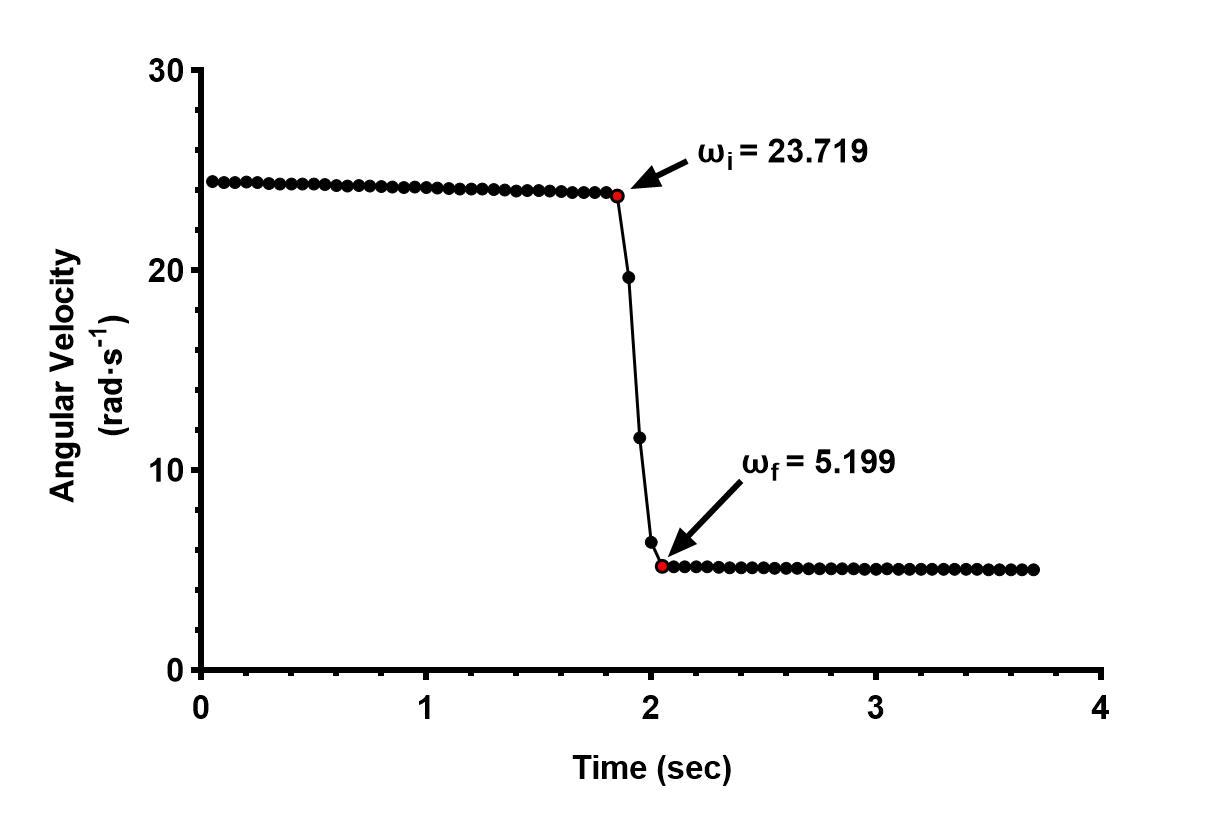
\includegraphics[width=\linewidth]{r3}
	\captionof{figure}{Ring (run 3)}
	\label{fig:test2}
\end{minipage}%
	\begin{minipage}{.5\textwidth}
	\centering
	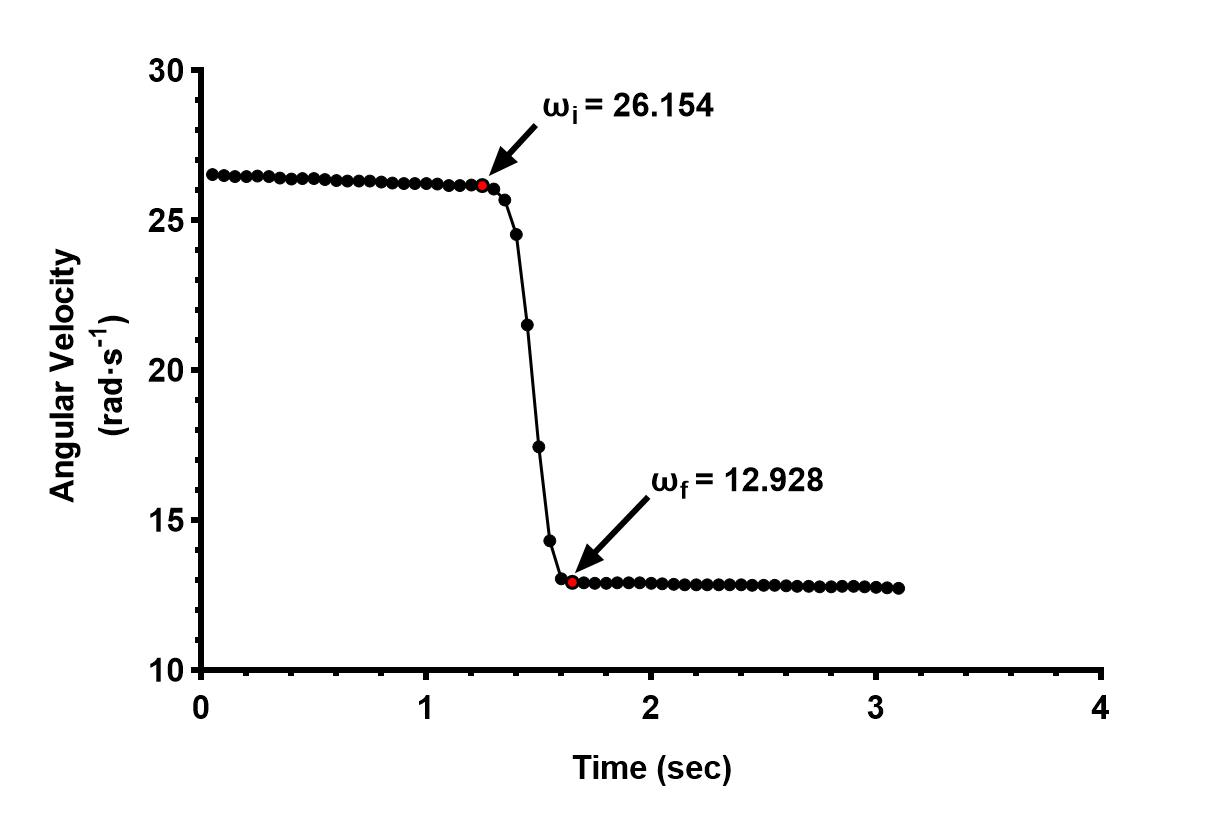
\includegraphics[width=\linewidth]{d}
	\captionof{figure}{Disk}
	\label{fig:test2}
\end{minipage}
\end{figure}
\newpage
.
\subsection{Derived Quantities}
We address the propogation error ($\delta$) for the derived variables in this experiment, by utilizing the following result. Given a derived variable $y=f(x_1,\cdots,x_m)$, the error in $y$ is
$$
\delta y=\sqrt{\sum_{i=1}^{m}\left(\frac{\partial f}{\partial x_{i}}\right)^{2}\left(\delta x_{i}\right)^{2}}.$$

From this, we obtain the following results.

\begin{table}[!htb]
	\centering
	\begin{tabular}{@{}lll@{}}
		\toprule
		Dropped Object & $I_i$ (gcm$^2$) & $I_f$ (gcm$^2$) \\ \midrule
		\multicolumn{1}{l|}{Ring (run 1)} & \multicolumn{1}{l|}{1407$\ \pm 4$} & 6461$\ \pm 8$ \\
		\multicolumn{1}{l|}{Ring (run 2)} & \multicolumn{1}{l|}{1407$\ \pm 4$} & 6463$\ \pm 8$ \\
		\multicolumn{1}{l|}{Ring (run 3)} & \multicolumn{1}{l|}{1407$\ \pm 4$} & 6464$\ \pm 8$ \\
		\multicolumn{1}{l|}{Disk} & \multicolumn{1}{l|}{1407$\ \pm 4$} & 2831$\ \pm 7$ \\ \bottomrule
	\end{tabular}
\caption{Collision Data: Moment of Inertia}
\end{table}


% Please add the following required packages to your document preamble:
% \usepackage{booktabs}
\begin{table}[!htb]
	\centering
	\begin{tabular}{@{}llll@{}}
		\toprule
		Dropped Object & $L_i$ (gm$^2$/s) & $L_f$ (gm$^2$/s) & \% diff \\ \midrule
		\multicolumn{1}{l|}{Ring (run 1)} & \multicolumn{1}{l|}{3.6621$\ \pm0.0152$} & \multicolumn{1}{l|}{3.6130$\ \pm0.0049$} & $-$1.34 \\
		\multicolumn{1}{l|}{Ring (run 2)} & \multicolumn{1}{l|}{3.2908$\ \pm0.0137$} & \multicolumn{1}{l|}{3.3091$\ \pm0.0041$} & +0.56 \\
		\multicolumn{1}{l|}{Ring (run 3)} & \multicolumn{1}{l|}{3.3616$\ \pm0.0144$} & \multicolumn{1}{l|}{3.3606$\ \pm0.0044$} & $-$0.03 \\
		\multicolumn{1}{l|}{Disk} & \multicolumn{1}{l|}{3.6644$\ \pm0.0153$} & \multicolumn{1}{l|}{3.6599$\ \pm0.0051$} & $-$0.12 \\ \cmidrule(r){1-4}
	\end{tabular}
\caption{Collision Data: Angular Momentum}
\end{table}

\begin{table}[!htb]
	\centering
	\begin{tabular}{@{}llll@{}}
		\toprule
		Dropped Object & $\text{KE}_i$ (gm$^2$/s$^2$) & $\text{KE}_f$ (gm$^2$/s$^2$) & \% diff \\ \midrule
		\multicolumn{1}{l|}{Ring (run 1)} & \multicolumn{1}{l|}{47.659$\ \pm0.191$} & \multicolumn{1}{l|}{10.102$\ \pm0.015$} & $-$78.80\\
		\multicolumn{1}{l|}{Ring (run 2)} & \multicolumn{1}{l|}{38.485$\ \pm0.133$} & \multicolumn{1}{l|}{8.475$\ \pm0.009$} & $-$77.98 \\
		\multicolumn{1}{l|}{Ring (run 3)} & \multicolumn{1}{l|}{40.158$\ \pm0.137$} & \multicolumn{1}{l|}{8.736$\ \pm0.011$} & $-$78.25 \\
		\multicolumn{1}{l|}{Disk} & \multicolumn{1}{l|}{47.718$\ \pm0.193$} & \multicolumn{1}{l|}{19.897$\ \pm0.038$} & $-$58.30 \\ \bottomrule
	\end{tabular}
\caption{Collision Data: Rotational Kinetic Energy}
\end{table}
\section{Conclusion}
Data obtained in \textbf{Table 6} and \textbf{Table 7} strongly supports the validity of \textbf{Theorem 1.} The angular momentum is likely conserved in a torque-free system, as four runs all exhibit very minor difference ($<$2\%) in angular momentum before and after the collision. We also find that the rotational kinetic energy is not conserved during collision. Instead, it plummets to approximately a fifth of the initial value in the ring-disk system, and two fifths in the disk-disk system. This was possibly because the rotational kinetic energy was transformed into other forms of energy during the inelastic collision.

However, despite the successful verification of the physical law, improvements can still be made upon the design of the experiment. First, all moves of dropping the ring (disk) are done manually in the current experiment. The unstableness of the hands can easily translate to undesired movements (e.g., tilting) of the ring (disk). This dramatically increases the difficulty of the experiment. A mechanical device could be helpful in releasing the load in a more controlled and predictable manner. Second, it is noticed that after releasing and striking the disk, the ring is very likely to bump off the center of the disk. The current solution involves measuring the displacement of the ring from the edge of the disk. But this was undeniably hard and inaccurate, introducing significant uncertainty to the result. To address this problem, we can create a shallow, ring-shaped trough on the surface of the disk that helps lock the ring in place. 



\end{document}